\documentclass[11pt]{article}
\usepackage[margin=1in]{geometry}
\usepackage{amsmath,amssymb,amsfonts,bm}
\usepackage{booktabs}
\usepackage{graphicx}
\graphicspath{{../}}
\usepackage{hyperref}
\usepackage{xcolor}

\title{Basin Stability v7: Two-Replica Edwards--Anderson\\
       Order Parameter and Phase Classification}
\author{}
\date{}

\begin{document}
\maketitle

\section{Overview}

Version~7 of the basin stability protocol extends v6 by simultaneously computing two observables on the $(\alpha, T)$ grid:
\begin{itemize}
    \item \textbf{Alignment} $\varphi(\alpha, T) = \langle \boldsymbol{\xi}^1 \!\cdot\! \mathbf{x} / N \rangle$ --- overlap with the stored pattern (as in v6).
    \item \textbf{Edwards--Anderson order parameter} $q_{\mathrm{EA}}(\alpha, T)$ --- a two-replica self-overlap that distinguishes frozen (glassy) from ergodic (paramagnetic) phases.
\end{itemize}

\section{Two-Replica Protocol}
\label{sec:two-replica}

For each disorder sample (pattern set), two replicas $\mathbf{x}_a$ and $\mathbf{x}_b$ are evolved independently under the same quenched disorder but with independent Monte Carlo noise. The replicas share the same patterns $\{\boldsymbol{\xi}^\mu\}$ and inverse temperatures $\beta = 1/T$, but are initialized with different random seeds and evolve along independent Markov chains.

After $n_{\mathrm{eq}}$ equilibration steps (unmeasured), both replicas are sampled for $n_{\mathrm{samp}}$ steps. At each sampling step:
\begin{align}
    \varphi_a &= \frac{\boldsymbol{\xi}^1 \!\cdot\! \mathbf{x}_a}{N}\,,\quad
    \varphi_b = \frac{\boldsymbol{\xi}^1 \!\cdot\! \mathbf{x}_b}{N}\,,\\[6pt]
    q_{\mathrm{EA}} &= \frac{\mathbf{x}_a \!\cdot\! \mathbf{x}_b}{N}\,.
\end{align}

The reported alignment is the average of both replicas over all sampling steps and disorder samples:
\begin{equation}
    \varphi(\alpha, T) = \Bigl\langle \frac{\varphi_a + \varphi_b}{2} \Bigr\rangle_{\!\mathrm{samp,\, dis}}\,.
\end{equation}
The Edwards--Anderson parameter is the cross-overlap averaged over sampling steps and disorder:
\begin{equation}
    q_{\mathrm{EA}}(\alpha, T) = \bigl\langle \mathbf{x}_a \!\cdot\! \mathbf{x}_b / N \bigr\rangle_{\!\mathrm{samp,\, dis}}\,.
\end{equation}

\subsection{Interpretation of $q_{\mathrm{EA}}$}

\begin{itemize}
    \item $q_{\mathrm{EA}} \approx 1$: Both replicas are trapped in the same state --- the system is \emph{frozen} (non-ergodic). This occurs in the retrieval and spin-glass phases.
    \item $q_{\mathrm{EA}} \approx 0$: The two replicas explore different regions of configuration space --- the system is \emph{ergodic}. This is the paramagnetic phase.
    \item Intermediate values indicate partial freezing or slow dynamics.
\end{itemize}

The key advantage of $q_{\mathrm{EA}}$ is that it distinguishes the spin-glass phase (frozen but no retrieval, $\varphi \approx 0$, $q \gg 0$) from the paramagnetic phase (ergodic, $\varphi \approx 0$, $q \approx 0$), which cannot be differentiated by the alignment~$\varphi$ alone.

\subsection{Equilibrium $q_{\mathrm{EA}}$ and the parabolic law}
\label{sec:q-parabolic}

In the retrieval state, each replica independently aligns with the stored pattern $\boldsymbol{\xi}^1$ up to thermal fluctuations in the perpendicular subspace:
\begin{equation}\label{eq:replica-decomp}
    \mathbf{x}_{a} = \varphi\, \boldsymbol{\xi}^1 + \sqrt{1 - \varphi^2}\;\sqrt{N}\;\hat{\mathbf{u}}_{a}^{\perp}\,,
\end{equation}
where $\hat{\mathbf{u}}_{a}^{\perp}$ is a unit vector in the $(N\!-\!1)$-dimensional subspace orthogonal to $\boldsymbol{\xi}^1$, and similarly for replica~$b$. Since the two replicas evolve with independent Monte Carlo noise, $\hat{\mathbf{u}}_{a}^{\perp}$ and $\hat{\mathbf{u}}_{b}^{\perp}$ are uncorrelated, so their dot product vanishes for large~$N$:
\begin{equation}
    q_{\mathrm{EA}} = \frac{\mathbf{x}_a \!\cdot\! \mathbf{x}_b}{N}
    = \varphi^2 + (1-\varphi^2)\,\frac{\hat{\mathbf{u}}_a^{\perp}\!\cdot\!\hat{\mathbf{u}}_b^{\perp}}{1}
    \;\xrightarrow{N\to\infty}\; \varphi^2\,.
\end{equation}
At thermal equilibrium with overlap $\varphi_{\mathrm{eq}}(T)$, the predicted inter-replica overlap is therefore
\begin{equation}\label{eq:q-eq}
    q_{\mathrm{eq}}(T) = \varphi_{\mathrm{eq}}(T)^2\,.
\end{equation}

This prediction is verified numerically to four-decimal accuracy: at $\alpha = 0.1$ (deep retrieval regime), $q_{\mathrm{EA}} / \varphi^2 = 1.0000 \pm 0.0005$ across all temperatures $T \in [0.025,\, 2.0]$.

\paragraph{Normalized scatter plot.}
Dividing $q_{\mathrm{EA}}$ by $\varphi_{\mathrm{eq}}(T)^2$ removes the trivial thermal decrease visible in the raw $q_{\mathrm{EA}}(\alpha, T)$ map (Figure~\ref{fig:phases}, top right). In the normalized scatter plot (Figure~\ref{fig:phases}, bottom right), points at $(\tilde\varphi,\, q_{\mathrm{EA}}/\varphi_{\mathrm{eq}}^2)$ should lie on the parabola
\begin{equation}\label{eq:parabolic-law}
    \frac{q_{\mathrm{EA}}}{\varphi_{\mathrm{eq}}^2} = \tilde\varphi^2\,,\quad
    \tilde\varphi \equiv \varphi / \varphi_{\mathrm{eq}}\,,
\end{equation}
if both replicas independently achieve the same reduced overlap~$\tilde\varphi$ with the pattern. This is indeed observed for both the Retrieval (R) and Mixed (M) phases, confirming that the mixed phase represents \emph{partial retrieval} --- the system is partially attracted to the pattern, and both replicas track it to the same degree. The paramagnetic (P) points fall below the parabola, indicating that the replicas have decorrelated beyond what partial alignment with the pattern would predict.

\subsection{Limitations: spin-glass detection}
\label{sec:sg-limitation}

The quantity $q_{12} = \mathbf{x}_a \!\cdot\! \mathbf{x}_b / N$ measured here is the \emph{inter-replica} overlap, not the Edwards--Anderson self-overlap $q_{\mathrm{EA}}^{\mathrm{(self)}} = \lim_{t\to\infty} \langle S_i(t)\, S_i(0) \rangle$ in the strict sense.
In a true spin-glass phase with many degenerate metastable states, the two replicas would generically fall into \emph{different} spurious minima. Since random points on $S^{N-1}(\sqrt{N})$ have overlap $\sim 0$, the inter-replica overlap would be $q_{12} \approx 0$ --- indistinguishable from the paramagnetic phase.

The initialization protocol partially mitigates this: both replicas start near the same stored pattern ($\varphi_{\mathrm{init}} \in [0.75, 1]$), so if a dominant alternative minimum exists near the retrieval basin, both replicas may slide into it, yielding $q_{12} > 0$ with $\varphi \approx 0$ (correctly classified as SG). However, this is not guaranteed in a landscape with many degenerate minima.

The observation of 0\% spin-glass cells in the LSR data is therefore consistent with two interpretations: (i)~the LSR model genuinely has no spin-glass phase (as argued on theoretical grounds), or (ii)~the protocol cannot detect it because the replicas fall into different spurious states.
To unambiguously detect a spin-glass phase, one would need to measure the self-overlap (time autocorrelation within a single replica) or the full overlap distribution~$P(q)$.

\section{Phase Classification}
\label{sec:phases}

Using the normalized overlap $\tilde\varphi = \varphi / \varphi_{\mathrm{eq}}(T)$, where $\varphi_{\mathrm{eq}}(T)$ is the theoretical equilibrium overlap at temperature~$T$, the $(\alpha, T)$ plane is classified into four phases:

\begin{table}[h]
\centering
\caption{Phase classification thresholds and definitions.}
\label{tab:phases}
\begin{tabular}{llll}
\toprule
Phase & Symbol & Condition & Physical meaning \\
\midrule
Retrieval      & R  & $\tilde\varphi > \varphi_R$ and $q > q_{\mathrm{th}}$ & Pattern retrieved, frozen \\
Mixed          & M  & $\varphi_M < \tilde\varphi \le \varphi_R$ and $q > q_{\mathrm{th}}$ & Partial overlap, frozen \\
Spin-glass     & SG & $\tilde\varphi \le \varphi_M$ and $q > q_{\mathrm{th}}$ & No retrieval, frozen \\
Paramagnetic   & P  & $q \le q_{\mathrm{th}}$ & Ergodic, no order \\
\bottomrule
\end{tabular}
\end{table}

\noindent
The threshold values used are:
\begin{align}
    q_{\mathrm{th}} &= 0.15  && \text{(frozen/ergodic boundary)}\,,\\
    \varphi_R &= 0.99  && \text{(retrieval/mixed boundary)}\,,\\
    \varphi_M &= 0.1   && \text{(mixed/spin-glass boundary)}\,.
\end{align}

The normalization by the equilibrium overlap $\varphi_{\mathrm{eq}}(T)$ accounts for the temperature dependence of the retrieval state. For the LSR kernel, $\varphi_{\mathrm{eq}}(T)$ is obtained by solving the quadratic equation
\begin{equation}
    (bT + 1)\, y^2 - (2 + T + Tb)\, y + T = 0\,,\quad y = 1 - \varphi\,,
\end{equation}
and for the LSE kernel by solving $\varphi = \tfrac{1}{2}(-T + \sqrt{T^2 + 4})$.

\section{Threshold Contour Lines}
\label{sec:contours}

The phase maps (Figure~\ref{fig:phases}) overlay three threshold contour lines extracted from the data by linear interpolation along the $\alpha$ axis at each temperature:
\begin{itemize}
    \item $\tilde\varphi = \varphi_R = 0.99$ (black dashed) --- retrieval boundary,
    \item $\tilde\varphi = \varphi_M = 0.1$ (green dashed) --- mixed/spin-glass boundary,
    \item $q_{\mathrm{EA}} = q_{\mathrm{th}} = 0.15$ (cyan dashed) --- frozen/ergodic boundary.
\end{itemize}

\noindent
Additionally, the theoretical phase boundary $\alpha_c(T)$ from the free-energy analysis is shown as a solid white curve:
\begin{equation}
    \alpha_c(T) = \tfrac{1}{2}\bigl[1 - f_{\mathrm{ret}}(T)\bigr]^2\,,
\end{equation}
where $f_{\mathrm{ret}}(T) = u(\varphi) - T\, s(\varphi)$ with $u(\varphi) = -(1/b)\ln[1 - b(1-\varphi)]$ and $s(\varphi) = \tfrac{1}{2}\ln(1-\varphi^2)$ for LSR.

Below $T_{\max}$ (the temperature at which $\alpha_c(T)$ reaches the zero-temperature critical capacity $\alpha_{\mathrm{th}} = \tfrac{1}{2}(1-1/b)^2$), the boundary becomes vertical at $\alpha = \alpha_{\mathrm{th}}$.

\section{Phase Maps}

\begin{figure}[h]
    \centering
    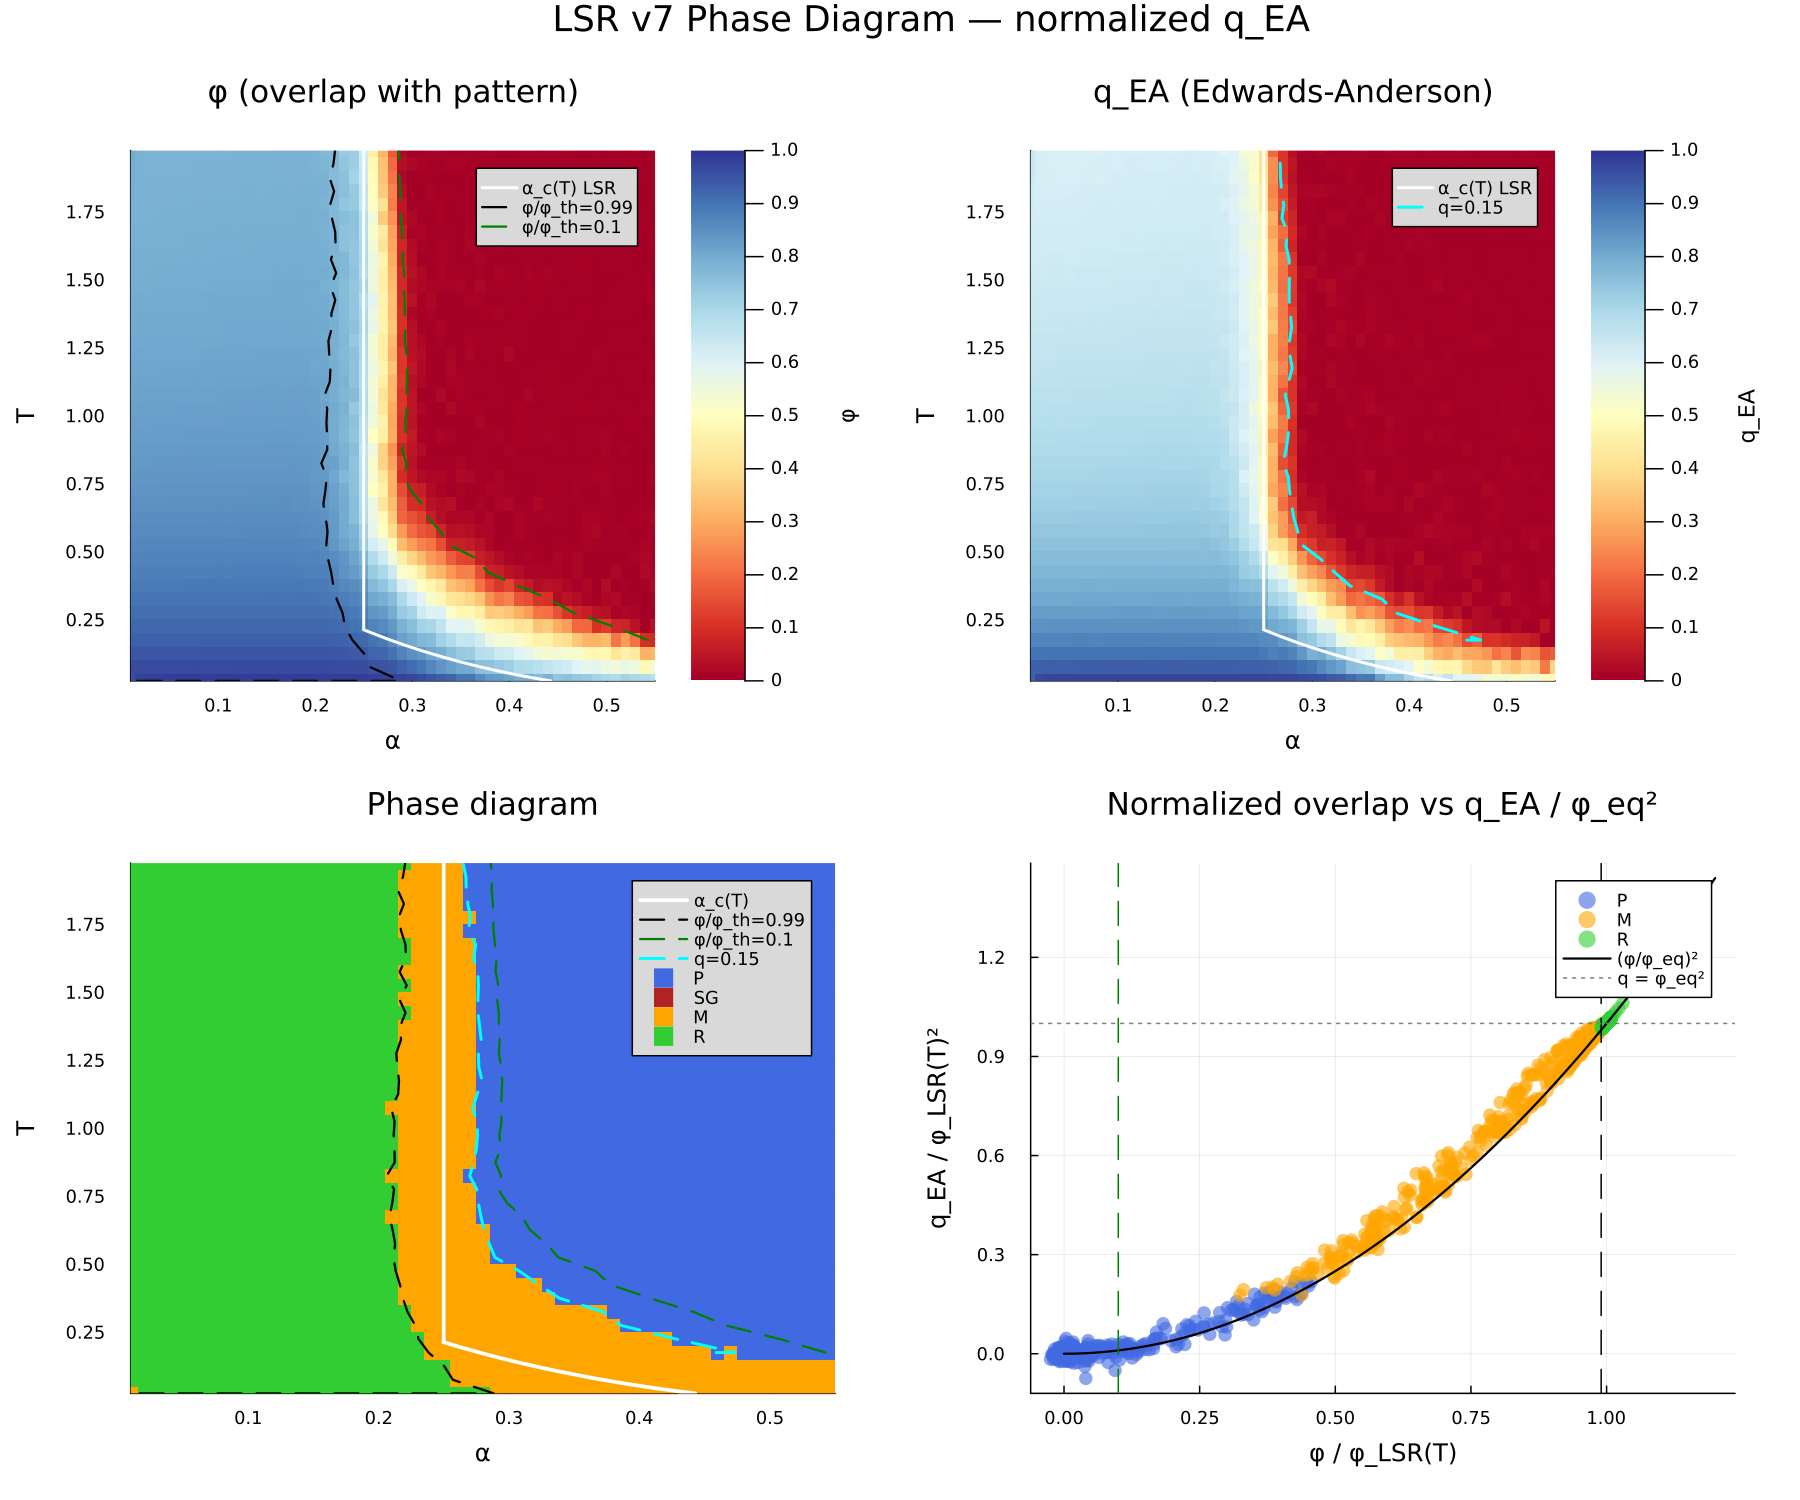
\includegraphics[width=0.99\textwidth]{maps_phases_LSR_v7_qnorm.png}
    \caption{LSR v7 phase diagram. \textbf{Top left:} alignment $\varphi(\alpha, T)$ with theoretical boundary (white) and threshold contour lines. \textbf{Top right:} Edwards--Anderson parameter $q_{\mathrm{EA}}(\alpha, T)$. \textbf{Bottom left:} four-phase classification (R~=~green, M~=~orange, SG~=~red, P~=~blue). \textbf{Bottom right:} normalized scatter plot of $\tilde\varphi = \varphi/\varphi_{\mathrm{eq}}$ vs.\ $q_{\mathrm{EA}}/\varphi_{\mathrm{eq}}^2$; the black curve is the parabolic law~\eqref{eq:parabolic-law} expected for two independent replicas at overlap~$\varphi$.}
    \label{fig:phases}
\end{figure}

\section{Simulation Parameters}

\begin{table}[h]
\centering
\caption{v7 Monte Carlo parameters (both LSE and LSR).}
\label{tab:v7-params}
\small
\begin{tabular*}{\textwidth}{@{\extracolsep{\fill}} l l}
\toprule
Parameter & Value \\
\midrule
$\alpha$ grid       & $0.01{:}0.01{:}0.55$ \;(55 values) \\
$T$ grid            & $0.025{:}0.05{:}2.0$ \;(40 values) \\
Initialization      & $\varphi_{\mathrm{init}} \sim \mathrm{U}(0.75,\, 1.0)$ \\
Equilibration       & $n_{\mathrm{eq}} = 2^{14} = 16{,}384$ steps (unmeasured) \\
Sampling            & $n_{\mathrm{samp}} = 2^{12} = 4{,}096$ steps ($\varphi$ and $q$ measured) \\
Trials              & $512 \to 64$ (linear in $\alpha$); two replicas per disorder sample \\
Step size           & $\sigma(N,T) = 2.4\, T / \sqrt{N}$ \\
Replicas            & 2 per disorder sample (shared patterns, independent MC) \\
Precision           & Float32 \\
\bottomrule
\end{tabular*}
\end{table}

\end{document}
